\section{Proposed experimental setup}\label{setup-section}
A dynamically polarized ${}^{14}$ND$_3$ target, described in the next Section, will provide the polarized neutrons on which the 11-GeV polarized electron beam from the upgraded CEBAF will be rastered.
In order to map the complex kinematic dependence of the GPDs, a wide acceptance detector is necessary. For this experiment, we plan to use the CLAS12 detector (Fig.~\ref{clas12}), which will be devoted to the detection of the electron, the neutron (in the Central Neutron Detector, described in Section \ref{cnd-section}) and the DVCS-BH photons. The CLAS12 acceptance for photons reaches down to polar angles of about $5^{\circ}$ with the Electromagnetic Calorimeter (EC). 
The possibility of extending the acceptance for photons down to $2.5^{\circ}$ using the electromagnetic calorimeter of the Forward Tagger (FT) \cite{batta} has been studied (Section \ref{ft_section}). As the results of these studies, which are not fully conclusive at this stage, show potential problems for the use of the FT at full luminosity, it will be used for a subset of the experiment (10 days), with half of the current. This will choice will be motivated and clarified in Section \ref{ft_section}. 
\begin{figure}
\begin{center}
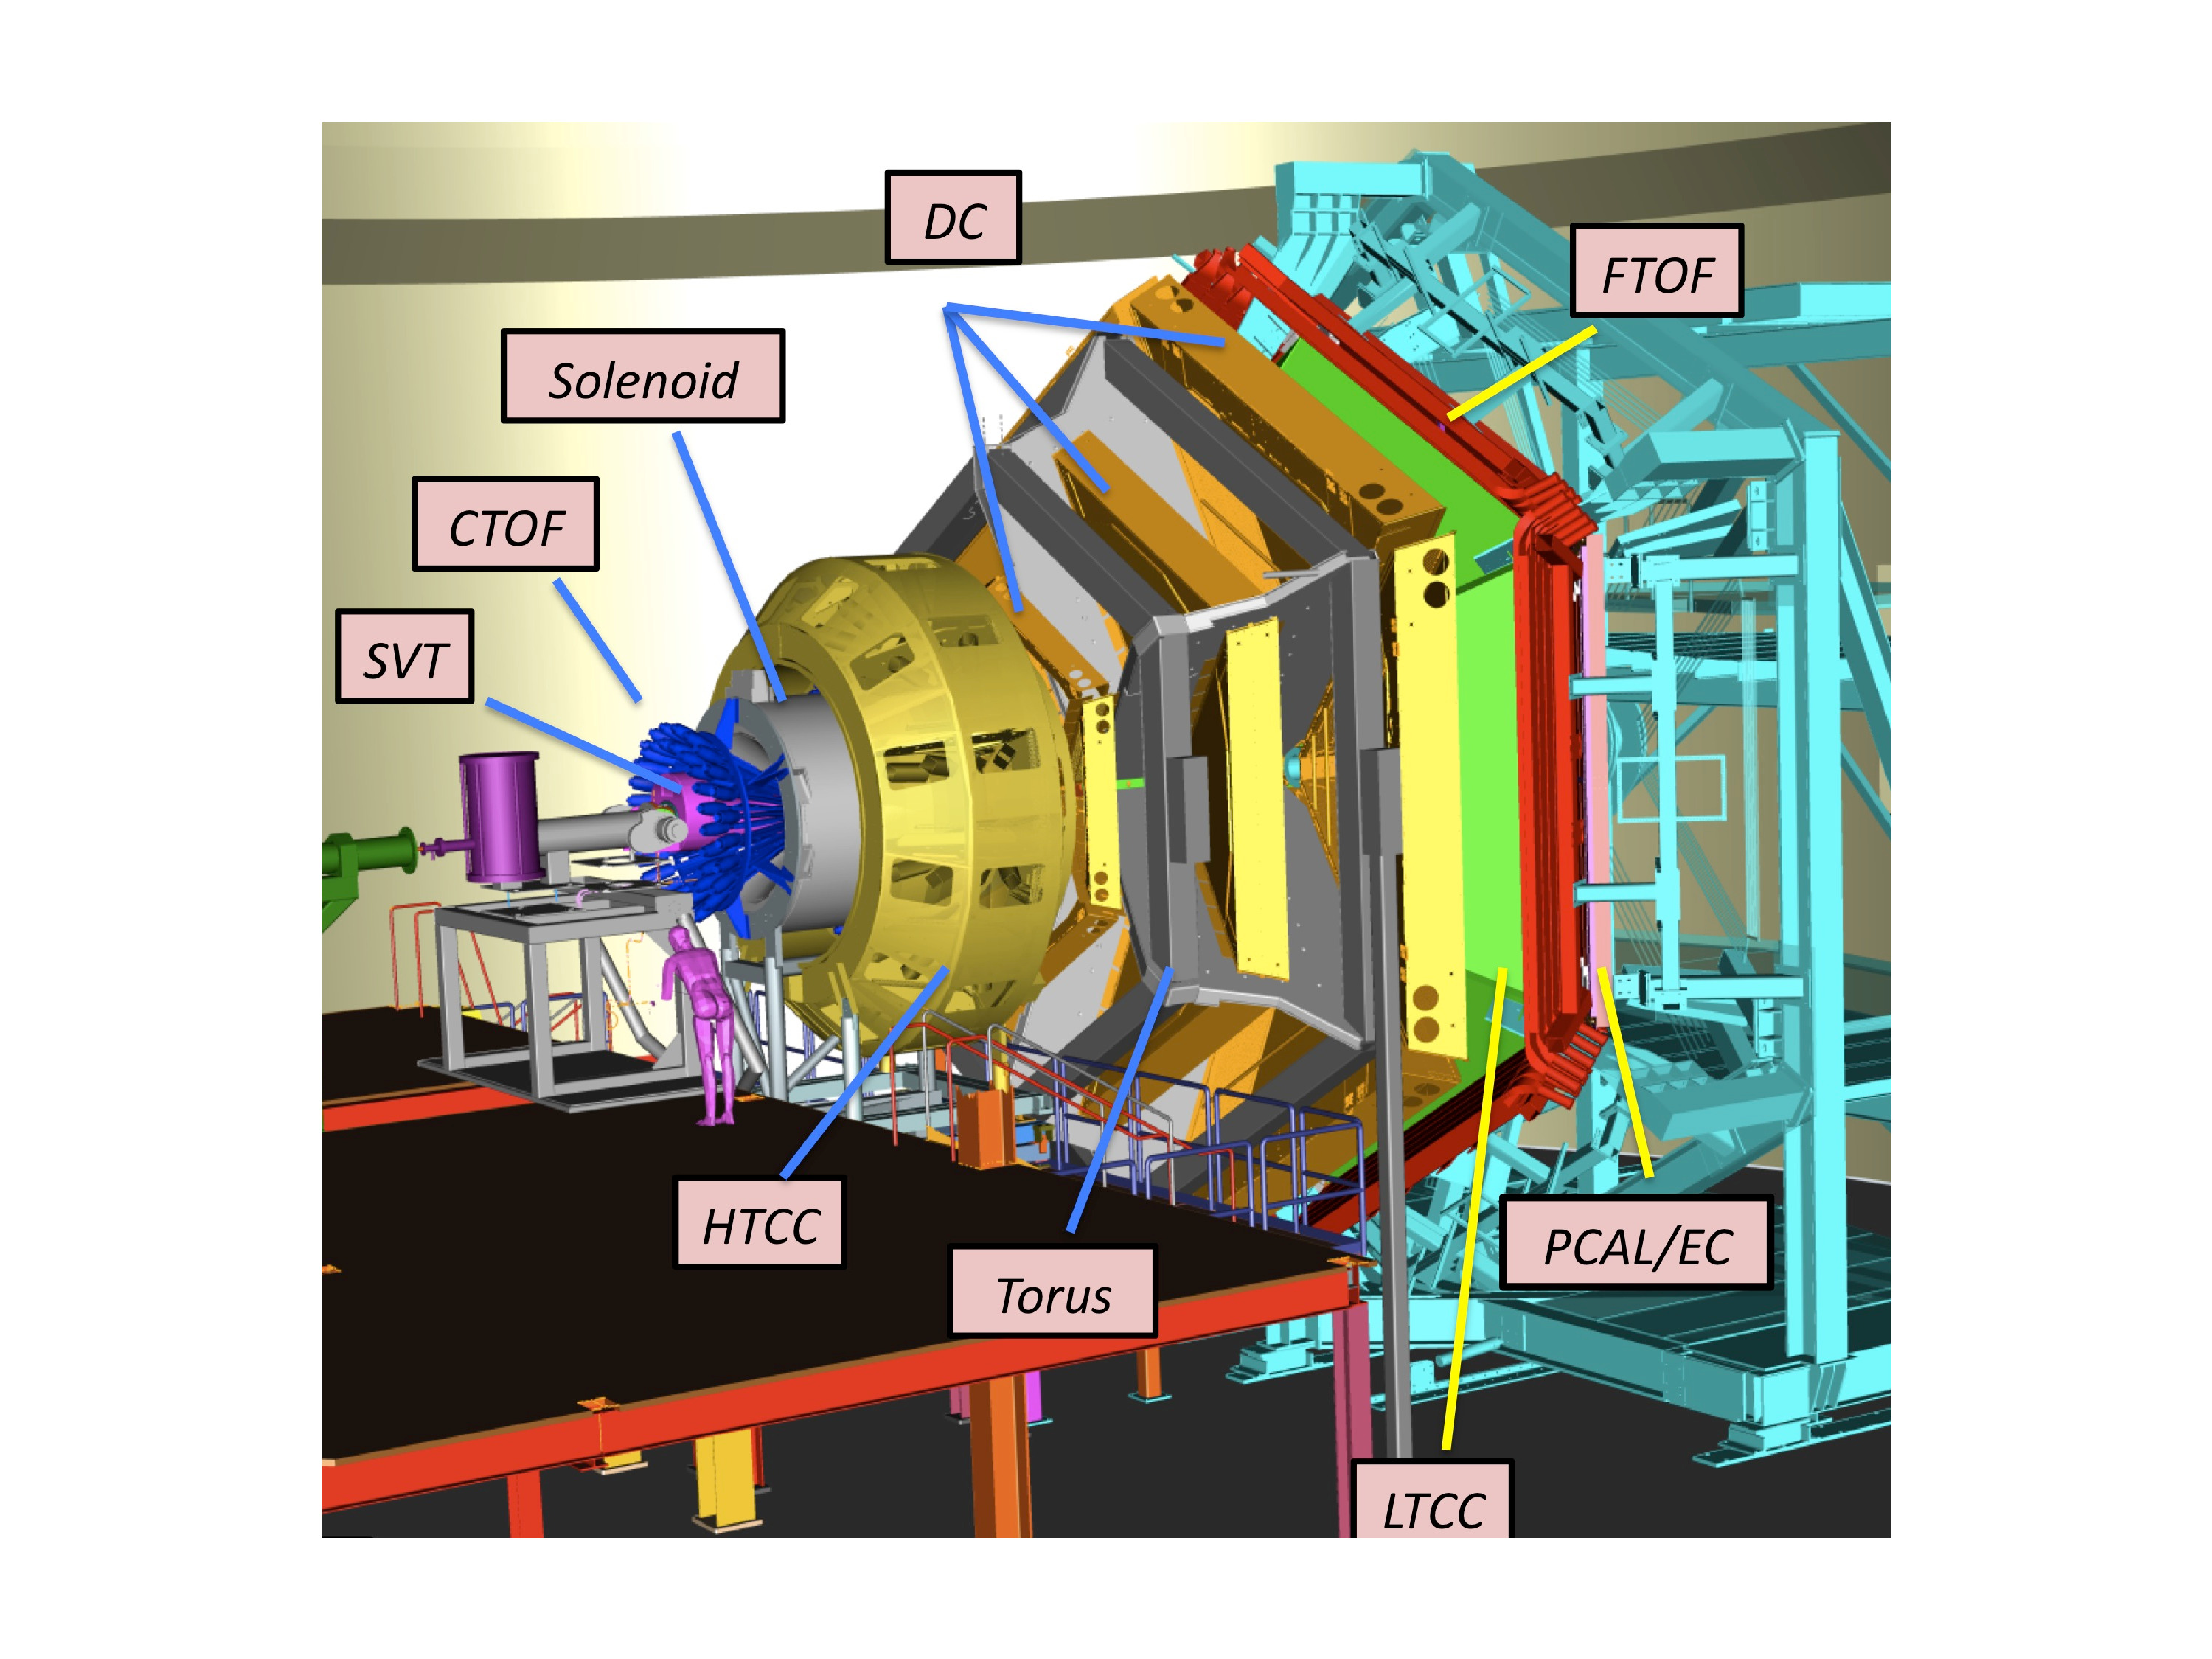
\includegraphics[width=130mm]{clas12-design.pdf}
\caption [The CLAS12 detector and its components]
{The CLAS12 detector and its components. In the forward part, the six coils of the superconducting toroidal magnet segment the detector into six sectors, each equipped with three regions of drift chambers (DC), High- and Low-Threshold Cherenkov Counters (HTCC and LTCC), Pre-Shower and Electromagnetic Calorimeters (PCAL and EC) and Forward Time-of-Flight (FTOF) scintillators. The central detector surrounds the target and is contained inside a solenoid magnet; its base equipment is composed of the Silicon Vertex Tracker (SVT) and the Central Time-of-Flight (CTOF).}
\label{clas12}
\end{center}
\end{figure}
